\documentclass[11pt]{article}
\usepackage[utf8]{inputenc}
\usepackage[T1]{fontenc}
\usepackage{minted}
\usepackage{graphicx}
\usepackage{hyperref}
\usepackage{CJKutf8}

\author{Student: Brian Cheung bc32427 \\ Professor: Mohit Tiwari \\ TA: Antonio Espinoza \\ Department of Electrical \& Computer Engineering \\ The University of Texas at Austin}
\date{\today}
\title{EE379K Enterprise Network Security Lab 2 Report}
\hypersetup{
 pdfauthor={Student: Brian Cheung bc32427 \\ Professor: Mohit Tiwari \\ TA: Antonio Espinoza \\ Department of Electrical \& Computer Engineering \\ The University of Texas at Austin},
 pdftitle={EE379K Enterprise Network Security Lab 2 Report},
 pdfkeywords={},
 pdfsubject={},
 pdfcreator={},
 pdflang={English}}

\begin{document}

\maketitle
\newpage
\section*{Part 1 - Vulnerable Web Apps}
\label{sec:part-1}
The task was to implement
\subsection*{1a - Set up a web-service in a container}
For this lab, the Damn Vulnerable Web App (DVWA) was set up as a web-service in a Docker container
using the following guide ~\cite{dvwa} and set to low difficulty.

\subsubsection*{PHP Injection}
The objective of this section was to implement a PHP injection that printed out the path to the current directory,
the contents of the current directory, the contents of the root of the file system, and the number of processes running in the system.
This was done by uploading a PHP script (part-1/php\_injection.php) to the DVWA and navigating to the file location.
The following image\ref{fig:php-injection} is the output of the script:
\begin{figure}[htbp]
  \centering
  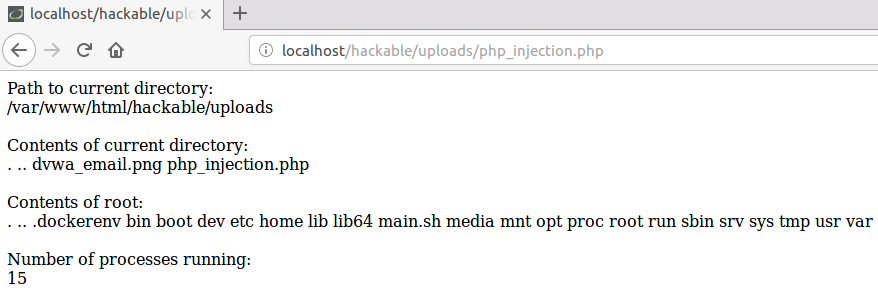
\includegraphics[width=.9\linewidth]{./php-injection.png}
  \caption{\label{fig:php-injection}
  Screenshot of the server's output after executing the PHP script.}
\end{figure}

\noindent Observations:
\begin{itemize}
  \item When running \verb|ls /| on the server and the VM, there are a few notable differences. The server shows some hidden files
  such as \verb|.|, \verb|..|, and \verb|.dockerenv|, while the VM does not. However, the VM displays some files and directories that the server doesn't such as
  \verb|cdrom/|, \verb|initrd.img|, \verb|initrd.img.old|, \verb|lost+found/|, \verb|core/|, \verb|snap/|, \verb|vmlinuz|, \verb|vmlinuz.old|.
  \item Running \verb=ps aux --no-headers | wc -l= from the VM's terminal resulted in 226 processes instead of the 15 processes when running the command on the server.
  \item These differences stem from the way Docker creates and manages containers. Docker uses cgroups to manage resource allocation
  and isolates the container's processes from the host machine through the use of namespaces.
  Each container also has its own root file system, which explains the different views of the filesystem when running \verb|ls /|.~\cite{codementor,demystify}
\end{itemize}

\subsection*{1b - Getting familiar with strace}
In order to detect a DVWA exploit, a tool called \verb|strace| was used to log all the system calls made by the container.
This can be done by attaching \verb|strace| to the process called \verb|containerd|, which executes the system calls on behalf of the Docker container.
To attach \verb|strace| to \verb|containerd|, the PID of \verb|containerd| must be passed as an argument to \verb|strace|.
\noindent To get the PID of \verb|containerd|, the following command was run in the terminal:
\begin{minted}{bash}
  $ ps -ef | grep containerd
  root      1155     1  0 09:36 ?        00:00:08 /usr/bin/containerd
\end{minted}
\noindent Then to monitor the system calls made by DVWA run the following command:
\begin{minted}{bash}
  $ sudo strace -p 1155 -o strace.txt -f
\end{minted}
\noindent Then run DVWA in a different terminal window:
\begin{minted}{bash}
  $ docker run --rm -it -p 80:80 vulnerables/web-dvwa
\end{minted}

\noindent For demonstration purposes, a bash command was injected into the input in the 'Command Injection' tab:
\begin{minted}{bash}
  ; echo "malware" > /tmp/maliciousfile
\end{minted}

The semi colon closes off the \verb|ping| command making the server run the bash command that follows.
The following lines identify the malicious sytem calls made during the exploit:
\begin{minted}{bash}
  28552 execve("/bin/sh", ["sh", "-c", "ping  -c 4 ; echo \"malware\" > /t"...], [/* 9 vars */] <unfinished ...>
  ...
  28552 open("/tmp/maliciousfile", O_WRONLY|O_CREAT|O_TRUNC, 0666) = 3
  28552 fcntl(1, F_DUPFD, 10)             = 10
  28552 close(1)                          = 0
  28552 fcntl(10, F_SETFD, FD_CLOEXEC)    = 0
  28552 dup2(3, 1)                        = 1
  28552 close(3)                          = 0
  28552 write(1, "malware\n", 8)          = 8
  28552 dup2(10, 1)                       = 1
  28552 close(10)                         = 0
  28552 exit_group(0)                     = ?
  28552 +++ exited with 0 +++
\end{minted}

\subsection*{1c - Limit who on the network can access the website using iptables}


\section*{Part 2 - SELinux}
\label{sec:part-1}
\subsection*{Policy Modules}
For this part of the lab, a simple policy module was created, and the file contexts were applied to the files and directories.
Then running the \verb|simple| executable, created a file, \verb|simple.txt|, with the \verb|simple_var_t| type.
The following figure shows the output of running \verb|ls -Z|:
\begin{figure}[htbp]
  \centering
  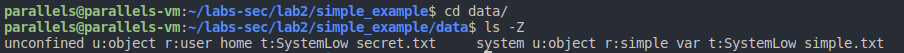
\includegraphics[width=.71\linewidth]{./ls-z.png}
  \caption{\label{fig:ls-z}
  Screenshot of the context of \verb|simple.txt|.}
\end{figure}

The following figure shows the error received when the \verb|simple| executable tries to read \verb|secret.txt| without the correct required permissions:
\begin{figure}[htbp]
  \centering
  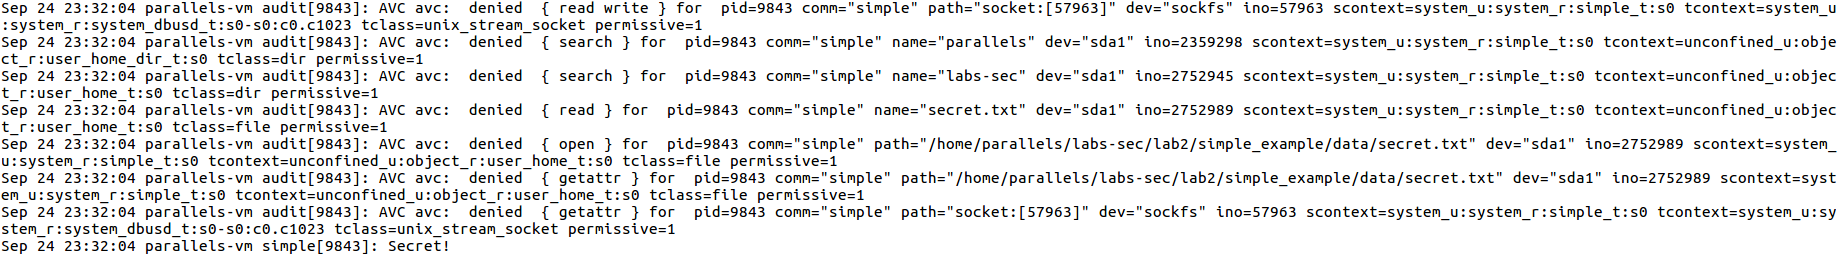
\includegraphics[width=.71\linewidth]{./log.png}
  \caption{\label{fig:log}
  Screenshot of log denying access to secret.txt.
\end{figure}

Context files (simple.fc) "declare the security contexts that are applied to files when the policy is installed"~\cite{context}.
Such security contexts include user, role, type, and level.
Type enforcement files (simple.te) define types and assign rules to each of the types.
Files associated with a specific type will have the permissions defined for that type.

\section*{Conclusion}
\label{sec:conclusion}
The lab took about 40 hours which was a bit longer than expected.
It was pretty interesting learning about socket connections in different languages and how GET requests are built using socket connections.
I think some parts of the lab were a little unclear and needed further clarification.
Overall, this lab served its purpose in providing a more hands-on experience that helped improve my understanding of networking.

\nocite{*}
\bibliography{bibliography}
\bibliographystyle{ieeetr}
\end{document}
